%%
%%
%% beamerthemethuas-doc.tex
%%
%% Definitions for the beamer layout for
%%
%% The Hague University of Applied Sciences (THUAS)
%%
%% (c)2021 J. op den Brouw  <J.E.J.opdenBrouw@hhs.nl>
%%
%%
%% This work may be distributed and/or modified under the
%% conditions of the LaTeX Project Public License, either version 1.3
%% of this license or (at your option) any later version.
%% The latest version of this license is in
%%   http://www.latex-project.org/lppl.txt
%% and version 1.3 or later is part of all distributions of LaTeX
%% version 2005/12/01 or later.
%%
%% This work has the LPPL maintenance status `maintained'.
%% 
%% The Current Maintainer of this work is J.E.J. op den Brouw
%%
%% This work consists of the files
%%   beamerthemethuas.sty
%%   beamerinnerthemethuas.sty
%%   beamerouterthemethuas.sty
%%   beamercolorthemethuas.sty
%%   beamerthemethuas-doc.tex
%%   beamerthemethuasfront.pdf
%%
%% and the derived file beamerthemethuas-doc.pdf
%%


%% Use ``dutch'' as class option
\documentclass[fleqn,aspectratio=169,dutch,10pt]{beamer}

%% Babel is needed for correct translations
%% It needs the ``dutch'' option
\usepackage[dutch]{babel}

%% Show frames, for testing
%\usepackage{showframe}

%% The THUAS beamer style, loads the correct fonts
\usetheme[nav,moreofficial]{thuas}

%% PGFplots
\usepackage{pgfplots}
\usepgfplotslibrary{fillbetween}
\usepgfplotslibrary{patchplots}
\pgfplotsset{compat=1.3}
%% Tikz already loaded by theme
\usetikzlibrary{spy}
\usetikzlibrary{backgrounds}
\usetikzlibrary{decorations}

\pgfdeclarelayer{background layer}
\pgfsetlayers{background layer,main}

%% Nice listings
\usepackage{listings}
\lstset{
    language=C,
    basicstyle=\ttfamily\small,
    xleftmargin=1em,
}

%% Nice tables, no vertical bars!
\usepackage{booktabs}

%% Typeset quantities in math mode
%\usepackage{siunitx}

%% Set up credentials
\title{THUAS Beamer Slides}
\subtitle{De THUAS layout maar nu met Beamer}
\author{Jesse op den Brouw}
\date{\today}

%%
%%
%%
\begin{document}

%% Title slide must not appear in a frame environment!
\maketitle


\begin{frame}[fragile]
\frametitle{THUAS Beamer Slides}
\begin{itemize}
\item This is the unofficial release of the Beamer theme for the The Hague University of Applied Science (THUAS)
\item First, load the beamer class: \lstinline|\documentclass{beamer}|
\item Next, load the theme with: \lstinline|\usetheme[|\emph{\small options}\lstinline|]{thuas}|
\item Works with \LaTeX, Xe\LaTeX en Lua\LaTeX
\item Works with Dutch and English
\item The remaining documentation is in Dutch
\end{itemize}
\end{frame}


\begin{frame}[fragile]
\frametitle{THUAS Beamer Slides}
\begin{itemize}
\item Dit is de onofficiële realisatie van slides met het THUAS-thema
\item Eerst gebruik je de beamer-class: \lstinline|\documentclass{beamer}|
\item Daarna laadt je de theme met: \lstinline|\usetheme[|\emph{\small opties}\lstinline|]{thuas}|
\item Het werkt met \LaTeX, Xe\LaTeX en Lua\LaTeX
\item Werkt met Nederlands en Engels
\item Gebruik \lstinline|\maketitle| voor de titelslide.
\begin{itemize}
\item Mag niet in een \lstinline|frame| environment!
\end{itemize}
\end{itemize}
\end{frame}


\begin{frame}[fragile]
\frametitle{THUAS Beamer Slides}
\begin{itemize}
\item De officiële realisatie is met aspect ratio 16:9, dus:
\begin{itemize}
\item Gebruik \lstinline|\documentclass[aspectratio=169]{beamer}|
\end{itemize}
\item Maar sommige beamers werken nog met 4:3, dus:
\begin{itemize}
\item Gebruik \lstinline|\documentclass[aspectratio=43]{beamer}|
\item Wordt niet actief ondersteund
\end{itemize}
\item Er zijn nog andere formaten maar die worden niet ondersteund
\item Er zijn verschillen in de titelslide tussen 16:9 en 4:3
\begin{itemize}
\item Dat komt o.a.\@ door het plaatsen van het plaatje op de titelslide
\end{itemize}
\item Er zijn verschillen tussen Xe-, Lua- en pdf\LaTeX
\begin{itemize}
\item Dat komt o.a.\@ door de vorm en de grootte van de gebruikte fonts
\end{itemize}
\end{itemize}
\end{frame}


\begin{frame}[fragile]
\frametitle{THUAS Beamer Slides}
\begin{itemize}
\item Nederlands en Engels worden ondersteund.
\item Nederlands is de standaard taal.
\begin{itemize}
\item Gebruik \lstinline|\usetheme[dutch]{thuas}|.
\item Op de titelslide en in de slides wordt dan het Nederlandse logo gebruikt.
\end{itemize}
\item Engels kan ook gebruikt worden.
\begin{itemize}
\item Gebruik \lstinline|\usetheme[english]{thuas}|.
\item Op de titelslide en in de slides wordt dan het Engelse logo gebruikt.
\end{itemize}
\end{itemize}
\end{frame}


\begin{frame}[fragile]
\frametitle{THUAS Beamer Slides}
\begin{itemize}
\item Standaard wordt 11pt fontgrootte gebruikt.
\item Dit kan je met een class optie aanpassen, bijvoorbeeld \lstinline|\documentclass[10pt]{beamer}|
\item Er zijn verschillende fontgroottes: 
\begin{itemize}
\item 8pt, 9pt, 10pt, 11pt (default), 12pt, 14pt, 17pt en 20pt.
\item 10pt en 11pt zijn de meest gangbare varianten.
\item 10pt komt het dichtst in de buurt van de PowerPoint-versie.
\item Voor 8pt, 9pt, 14pt, 17pt en 20pt moet de \lstinline|extsize| package geinstalleerd zijn.
\item Deze slides zijn gemaakt met 10pt.
\end{itemize}
\end{itemize}
\end{frame}


\begin{frame}[fragile]
\frametitle{THUAS Beamer Slides}
Om correct gebruik te maken van het Nederlands, gebruik
\begin{lstlisting}
\documentclass[dutch]{beamer}
\end{lstlisting}
en
\begin{lstlisting}
\usepackage[dutch]{babel}
\end{lstlisting}
Dan worden environments als \lstinline|theorem| en \lstinline|proof| van de correcte namen voorzien

%\alert{TODO}: automatisch laden van \lstinline|babel| met \lstinline|dutch| of \lstinline|english|
\end{frame}


\begin{frame}[fragile]
\frametitle{THUAS Beamer Slides}
Xe\LaTeX{} en Lua\LaTeX:
\begin{itemize}
\item Het standaard font is Arial voor lopende tekst en Arial Black voor titels
\item Het standaard font voor formules is Cambria Math
\item Het standaard font voor programmacode is Consolas
\item Deze fonts worden automatisch geladen
\item Voor Linux-gebruikers: zorg dat deze fonts beschikbaar zijn
\item Wil je andere fonts gebruiken, gebruik dan \lstinline|\usetheme[vanilla]{thuas}|
\end{itemize}
\end{frame}


\begin{frame}[fragile]
\frametitle{THUAS Beamer Slides}
pdf\LaTeX{}:
\begin{itemize}
\item Het standaard font is Helvet voor lopende tekst en Helvet/bold voor titels
\item Het standaard font voor formules is Libertinus Math
\item Het standaard font voor programmacode is Nimbus Mono
\item Deze fonts worden automatisch geladen
\item Wil je andere fonts gebruiken, gebruik dan \lstinline|\usetheme[vanilla]{thuas}|
\end{itemize}
\end{frame}


\begin{frame}[fragile]
\frametitle{THUAS Beamer Slides}
\begin{itemize}
\item Subtitel op titelslide wordt weergegeven
\begin{itemize}
\item Niet bij de originele setting
\end{itemize}
\item Subtitels op frames worden \emph{niet} weergegeven
\begin{itemize}
\item Deze subtitels worden gewoon genegeerd
\end{itemize}
\item De inhoud van een slide is \emph{top aligned}
\begin{itemize}
\item Dat is conform de huisstijl
\item Wil je toch gecentreerde slides, gebruik dan \lstinline|\usetheme[c]{thuas}|
\end{itemize}
\item Maak een allerlaatste slide met \lstinline|\beamerthemethuasbackframe|
\end{itemize}
\end{frame}


\begin{frame}[fragile]
\frametitle{THUAS Beamer Slides}
\begin{itemize}
\item Navigatie-buttons komen rechts boven
\begin{itemize}
\item Gebruik \lstinline|\usetheme[nav]{thuas}|
\end{itemize}
\item Als je handouts wilt maken, gebruik dan de \lstinline|handout| optie
\begin{itemize}
\item Gebruik \lstinline|\documentclass[handout]{beamer}|
\item Dit is een optie voor \lstinline|beamer|
\end{itemize}
\item Als je het totaal aantal slides naast het slidenummer wil gebruiken
\begin{itemize}
\item Gebruik \lstinline|\usetheme[numframes]{thuas}|
\item Beamer spreekt van \textsl{frames}
\item Werkt niet lekker met voetnoten
\end{itemize}
\end{itemize}
\end{frame}


\begin{frame}[fragile]
\frametitle{THUAS Beamer Slides}
\begin{itemize}
\item Er zijn diverse kleuren gedefinieerd.
\bigskip
\item \lstinline|thuasgreen| \textcolor{thuasgreen}{\rule{5pt}{5pt}}
\item \lstinline|thuasgrey| \textcolor{thuasgrey}{\rule{5pt}{5pt}}
\item \lstinline|thuasred| \textcolor{thuasred}{\rule{5pt}{5pt}}
\item \lstinline|thuasyellow| \textcolor{thuasyellow}{\rule{5pt}{5pt}}
\item \lstinline|thuasblue| \textcolor{thuasblue}{\rule{5pt}{5pt}}
\bigskip
\item Deze kunnen overal gebruikt worden waar een kleur nodig is.
\end{itemize}
\end{frame}


\begin{frame}[fragile]
\frametitle{THUAS Beamer Slides}
\begin{itemize}
\item De standaard kleur voor slide titel en logo is groen.
\item Je kan dit veranderen in THUAS grijs
\begin{itemize}
\item Gebruik \lstinline|\usetheme[grey]{thuas}|
\end{itemize}
\item Je kan dit veranderen in zwart
\begin{itemize}
\item Gebruik \lstinline|\usetheme[black]{thuas}|
\end{itemize}
\item De standaard kleur voor \emph{alerted} tekst is \lstinline|thuasred|.
\begin{itemize}
\item Dit kan aangepast worden: \lstinline|\setbeamercolor*{alerted text}{fg=thuasblue}|
\end{itemize}
\end{itemize}
\end{frame}


\beamerthemethuaslogofalse

\begin{frame}[fragile]
\frametitle{THUAS Beamer Slides}
\begin{itemize}
\item Standaard wordt het logo rechtsonder weergegeven, behalve bij de titelslide
\item Het logo kan je uitzetten met \lstinline|\beamerthemethuaslogofalse|
\item Het logo blijft dan uit
\item Het logo kan je aanzetten met \lstinline|\beamerthemethuaslogotrue|
\item Het logo blijft dan aan
\item Op deze slide is het logo uit
\end{itemize}
\end{frame}

\beamerthemethuaslogotrue


\begin{frame}[fragile]
\frametitle{THUAS Beamer Slides}
\begin{itemize}
\item Soms wil je een tweede titelslide maken, bijvoorbeeld voor de tweede les, maar de slides bij elkaar houden.
\item Gebruik gewoon \lstinline|\maketitle|:
\begin{lstlisting}
\subtitle{Tweede les: kwantumfysica}
\author{N. Bohr en A. Einstein}
\maketitle
\end{lstlisting}
\item Het logo en het slidenummer worden dan onderdrukt.
\item \lstinline|\maketitle| mag niet in een \lstinline|frame| environment!
\end{itemize}
\end{frame}


\begin{frame}[fragile]
\frametitle{THUAS Beamer Slides}
\begin{itemize}
\item Verschillende offici\"ele versies.
\item Gebruik \lstinline|\usetheme[official]{thuas}| voor een offici\"ele titelslide.
\begin{itemize}
\item Is de default waarde, dus je kan het ook weglaten.
\end{itemize}
\item Gebruik \lstinline|\usetheme[moreofficial]{thuas}| om aan de linkerkant de THUAS-groene polygon te krijgen.
\begin{itemize}
\item De polygon schuift mee met de plaats van de titel.
\end{itemize}
\item Gebruik \lstinline|\usetheme[reallyofficial]{thuas}| om ook nog een \textsl{transfade} tussen twee slides te krijgen.
\end{itemize}
\end{frame}


\begin{frame}
\frametitle{Formules kunnen ook}
\begin{itemize}
\item De formules zijn (met behulp van een \lstinline|align*| environment):
\begin{align*}
\left|F(x)\right|^b_a &= \int_a^b x^2 + 2x + 1 \, \mathrm{d} x \\
\zeta (s) &= \sum_{n=1}^\infty \dfrac{1}{n^{s}} \\
M&\approx\frac{\pi}{4}\left(\frac{2d}{\lambda_o}\right)^2\left(\mathrm{NA}\right)^2
\end{align*}
\end{itemize}
\end{frame}


\begin{frame}
\frametitle{Formules kunnen ook}
Nu zonder itemize (met behulp van \lstinline|equation*| en \lstinline|multiline*|)
\begin{equation*}
\tan \alpha = \dfrac{\sin \alpha}{\cos \alpha} \qquad \tan x = \sin x \, / \cos x
\end{equation*}%
\begin{multline*}  
K=\displaystyle{\frac{1}{2}m_1 L_1^2 \dot{\theta_1}^2+\frac{1}{2} m_2[L_1^2 \dot{\theta_1}^2+L_2^2 \dot{\theta_2}^2+2 L_1 L_2 \dot{\theta_1}\dot{\theta_2}\cos(\theta_1-\theta_2)]} \\
 \displaystyle{+\frac{1}{2}m_3[L_1^2 \dot{\theta_1}^2+L_2^2 \dot{\theta_2}^2+L_3^2+ \dot{\theta_3}^2+2 L_1 L_2 \dot{\theta_1}\dot{\theta_2}\cos(\theta_1-\theta_2)}
\end{multline*}%
\begin{equation*}
\mathrm{e}^{\, \mathrm{j}\alpha} = \cos \alpha + \mathrm{j} \sin \alpha
\end{equation*}
\end{frame}


\begin{frame}
\frametitle{Voorbeeld met een itemize}
Voorbeeld met een \texttt{itemize} en gaat tot drie niveaus diep.
\begin{itemize}
\item item
\item item
\begin{itemize}
\item sub item
\item sub item
\begin{itemize}
\item sub sub item
\item sub sub item
\end{itemize}
\end{itemize}
\item item
\end{itemize}
Meer niveaus zijn in \lstinline|beamer| niet mogelijk.
\end{frame}


\begin{frame}
\frametitle{Voorbeeld met een enumerate}
Voorbeeld met een \texttt{enumerate} en gaat tot drie niveaus diep.
\begin{enumerate}
\item een
\item twee
\begin{enumerate}
\item een
\item twee
\begin{enumerate}
\item een
\item twee
\end{enumerate}
\end{enumerate}
\item drie
\end{enumerate}
Meer niveaus zijn in \lstinline|beamer| niet mogelijk.
\end{frame}


\begin{frame}
\frametitle{Voorbeeld van een description}
De label wordt vet en rechts uitgelijnd afgedrukt

De label kan ongeveer 9 karakters bevatten

Daarna wordt er ingesprongen
\begin{description}
\item[123456789] Dit is een hele lange tekst en ik denk dat deze zin over twee regels verspreid zal zijn
\item[label] description
\item[deze label is te groot] description
\end{description}
\end{frame}


\begin{frame}[fragile]
\frametitle{Tekst korter maken}
\begin{itemize}
\item Om tekst korter te maken zodat je aan de rechterkant nog ruimte over hebt voor een plaatje (of Ti\emph{k}z-figuur), gebruik dan \lstinline|minipage|. Zie het voorbeeld hieronder.
\end{itemize}
\bigskip
\begin{minipage}{0.5\linewidth}
\begin{itemize}
\item In het geheugen is er nu een stukje ruimte 
vrijgemaakt en deze heeft de naam a.
\item Met behulp van een toekenning kun je waardes 
stoppen in deze variabele:
\begin{lstlisting}[caption=]
a = 26;
\end{lstlisting}
\end{itemize}
\end{minipage}\hfil%
\begin{minipage}{0.2\linewidth}
\begin{tikzpicture}
\centering
\node[above] at (1,3) {computergeheugen};
\draw[fill=thuasgreen!30!white] (0,0) rectangle (2,3);
\node [draw, thick, shape=rectangle, minimum width=1cm, minimum height=0.5cm, anchor=center, fill=white] at (1.0,1.5) {\footnotesize 26} node[yshift=13] at (1.0,1.5) {\footnotesize a};
\end{tikzpicture}
\end{minipage}
\end{frame}


%% A frame with a listing NEEDS fragile
\begin{frame}[fragile]
\frametitle{Een frame met code}
Een frame met daarin code met \texttt{lstlistings} moet getypeerd worden met \texttt{fragile}, anders werkt het niet

\begin{lstlisting}
\begin{frame}[fragile]{Titel}
\end{lstlisting}

Voorbeeld:

\begin{lstlisting}
#include <stdio.h>

int main(void) {
    printf("THUAS Beamer Slides!\n");
}
\end{lstlisting}

Moet gebruikt worden voor alle verbatim code! Niet getest met \lstinline|minted|
\end{frame}


\begin{frame}[fragile]
\frametitle{Codefragment stap voor stap}
Een codefragment stap voor stap laten zien, kan door binnen een \lstinline|listing| de optie \lstinline|mathescape| te gebruiken. Zet de listing als volgt op:
\begin{lstlisting}[caption=]
\begin{lstlisting}[mathescape]
\end{lstlisting}
en gebruik daarna \lstinline|$\pause$| aan het begin van elke regel. Witregels kunnen zonder de pauze. Let op: je kan nu geen \lstinline|$| gebruiken in je code!
\begin{lstlisting}[caption=,mathescape]
int main(void)
$\pause${
$\pause$   int i = 5;

$\pause$   printf("i = %d\n", i);

$\pause$   return 0;
$\pause$}
\end{lstlisting}
\end{frame}


\begin{frame}[fragile]
\frametitle{Voetnoot en plaatje}
Een voetnoot\footnote{Dit is een voetnoot}. Gebruik liever geen voetnoot.

Een plaatje (met een \lstinline|\fbox| en \lstinline|\fboxsep=0pt|)

\begin{figure}
\fboxsep=0pt
\fbox{\resizebox{0.30\paperwidth}{!}{\beamerthemethuaslogo}}
\caption{Dit is een plaatje}
\end{figure}

De fontgrootte van de caption is \lstinline|\footnotesize|.

\end{frame}


\begin{frame}[fragile]
\frametitle{Tabellen}
Een tabel kan ook (deze is met \texttt{booktabs})

\begin{table}[!ht]
\caption{Een tabel}
\begin{tabular}{llcc}
\toprule
Iets & En nog iets & Bla & Bla \\
\midrule
Aaa & Bbb & 1.24 & 2.54 \\
Aaa & Bbb & 1.24 & 2.54 \\
Aaa & Bbb & 1.24 & 2.54 \\
\bottomrule
\end{tabular}
\end{table}

Let op: \texttt{siunitx} typesets in math-mode!

De fontgrootte van de caption is \lstinline|\footnotesize|.
\end{frame}


\begin{frame}
\frametitle{De normaalverdeling met \texttt{pgfplots} (Kees!)}
\begin{figure}
\begin{tikzpicture}[
  declare function = { bell(\x) = exp(-\x^2); }
  ]
\begin{axis}[
    width=0.7\paperwidth,
    height=0.65\paperheight,
    xtick={-4.0,-3.0,-2.0,-1.0,0.0,1.0,2.0,3.0,4.0}, 
    xticklabels={$-4\sigma$, $-3\sigma$, $-2\sigma$, $-1\sigma$, $0$, $1\sigma$, $2\sigma$, $3\sigma$, $4\sigma$},
    font=\footnotesize
  ]

%% Plot bell curve
\addplot [thuasgreen!50!black, mark=none, samples=301, name path=f,domain=-4:4] { bell(\x) };

%% Just a path over the x axis
\path[name path=xaxis] (axis cs:-4,0) -- (axis cs:4,0);

%% Fill the area between x axis and bell curve, from x = -1 to x = 1 (1 sigma)
\addplot [thick, fill=thuasgreen, fill opacity=0.25]
              fill between[of=f and xaxis, soft clip={domain=-1:1}];
        
%% Draw the 1 sigma from-to line, set text in math mode
\draw[latex-] (axis cs:0.0,0.4) -- (axis cs:1.1,0.75) node[right] {Area is 68.26\,\% of total};

\draw[latex-] (axis cs:-0.7,{bell(-0.7)}) -- (axis cs:-2,0.8) node[left] {$\mathrm{e}^{-x^2}$};
\end{axis}
\end{tikzpicture}
\end{figure}
\end{frame}


\begin{frame}
\frametitle{Een 3D-plaatje met \texttt{pgfplots}}
\begin{figure}
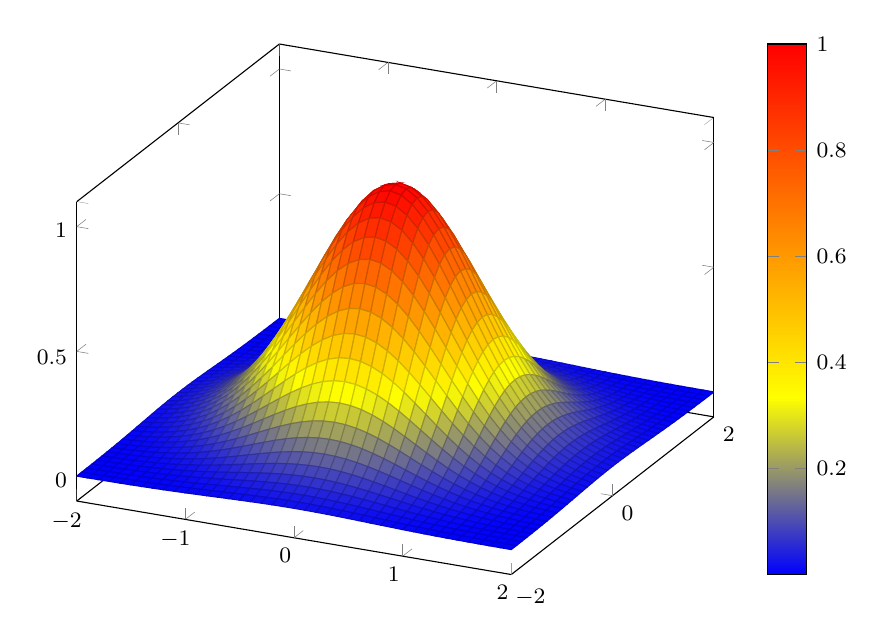
\begin{tikzpicture} 
\begin{axis}[
   colorbar,
   colorbar style={
     font=\footnotesize
   },
   width=0.45\paperwidth,
   font=\footnotesize,
]
  \addplot3[surf,samples=41,domain=-2:2] {exp(-x^2-y^2)};
\end{axis}
\end{tikzpicture}
\end{figure}
\end{frame}


\begin{frame}
\frametitle{Afgeleide met \texttt{spy}, \texttt{decorations} \& \texttt{background}}
\def\ll{1.0}
\def\rr{2.0}
\centering
\begin{tikzpicture}
  [line cap=round,line join=round,scale=1,
     %using the 'spy' to magnify a part of the picture
     spy using outlines={circle,lens={scale=1.5}, size=4cm, connect spies},
     %using the decoration 'brace' (=a curly brace as path replacement)
     decoration={brace,amplitude=2pt},
	 declare function={ f(\x) = (0.3*\x*\x);}
  ]

  \coordinate (leftc) at (\ll,{f(\ll)});
  \coordinate (rightc) at (\rr,{f(\rr)});
  \coordinate (meet) at (\rr,{f(\ll)});

  \draw[domain=0:3,thick] plot (\x,{f(\x)}) node[below right] {$f(x)$};
  \draw[red] (leftc) circle (1pt) node[above left, black] {$A$};
  \draw[red] (rightc) circle (1pt) node[above left, black] {$B$};
  \draw[blue,shorten >=-1cm,shorten <=-1cm] (leftc) -- (rightc);

  \draw [decorate,decoration={brace,mirror,amplitude=4pt},color=green!30!black] (leftc)--(meet)
        node [midway,anchor=north,inner sep=5pt, outer sep=1pt]{$\Delta x$};

  \draw [decorate,decoration={brace,amplitude=4pt},color=violet] (rightc)--(meet)
        node [midway,anchor=west,inner sep=5pt, outer sep=1pt]{$\Delta y$};

  \spy [brown] on (1.6,0.6) in node [left] at (9.5,1);

  \begin{pgfonlayer}{background layer}
    \fill[yellow!20] (-0.5,-1) rectangle (4,3);
  \end{pgfonlayer}
\end{tikzpicture}
%
\begin{equation*}
%\lim_{\Delta x\rightarrow 0}f(x + \Delta x) = \dfrac{\mathrm{d}f(x)}{\mathrm{d}x}
\end{equation*}
\end{frame}

\begin{frame}[fragile]
\frametitle{Gory details...}
De theme package bestaat uit:
\begin{itemize}
\item \texttt{beamerthemethuas.sty}
\begin{itemize}
\item Deze moet je aanroepen met \lstinline|\usetheme[|\textsl{opties}\lstinline|]{thuas}|
\item Deze package definieert een aantal macro's
\end{itemize}
\item \texttt{beamercolorthemethuas.sty}
\begin{itemize}
\item Hierin zijn de kleuren gedefinieerd. Deze kan je aanroepen.
\end{itemize}
\item \texttt{beamerinnerthemethuas.sty}
\begin{itemize}
\item Hierin is de opmaak \emph{van} de inhoud gedefinieerd (ook de titelslide). Niet aanroepen.
\end{itemize}
\item \texttt{beamerouterthemethuas.sty}
\begin{itemize}
\item Hierin is de opmaak \emph{rond} de inhoud gedefinieerd (header, footer). Niet aanroepen.
\end{itemize}
\end{itemize}
\end{frame}


\begin{frame}[fragile]
\frametitle{Gory details...}
Er wordt \'e\'en plaatje gebruikt
\begin{itemize}
\item Plaatje op titelslide: \lstinline|beamerthemethuasfront.pdf|
\item De logo's worden in PGF afgebeeld
\item []
\item De positie van de titel op een frame wordt getypeset door drie \lstinline|length|s
\begin{itemize}
\item \lstinline|\beamerthemethuastitleoffset|: offset vanaf de bovenkant, 0.7 cm
\item \lstinline|\beamerthemethuastitleheight|: hoogte van de titel, 2.25 ex
\item \lstinline|\beamerthemethuastitledepth|: diepte van de titel, 2.5 ex
\item Gebruik \lstinline|\setlength{...}{...}| om een \lstinline|length| aan te passen
\item De THUAS-polygon links schuift mee met de plaats van de titel.
\end{itemize}
\end{itemize}
\end{frame}


\begin{frame}
\frametitle{There Is No Largest Prime Number} 
\begin{theorem}
There is no largest prime number.
\end{theorem} 
\begin{proof}
\begin{enumerate} 
\item<1-| alert@1> Suppose $p$ were the largest prime number. 
\item<2-> Let $q$ be the product of the first $p$ numbers. 
\item<3-> Then $q+1$ is not divisible by any of them. 
\item<1-> But $q + 1$ is greater than $1$, thus divisible by some prime
number not in the first $p$ numbers.
\end{enumerate}
\end{proof}
\end{frame}


\begin{frame}[fragile]
\frametitle{Weetjes}
\begin{itemize}
\item Om ervoor te zorgen dat bij \lstinline|lstlisting| geen ruimte n\'a de code volgt, gebruik dan
\lstinline|\begin{lstlisting}[caption=]|
\item Om extra ruimte te laten tussen twee \lstinline|item|s, gebruik \lstinline|\item []|
\begin{itemize}
\item Of gebruik \lstinline|medskip|, \lstinline|bigskip|
\end{itemize}
\item Gebruik \lstinline|\usepackage{parskip}| niet! De interline ruimte wordt dan aangepast
\item Gebruik \lstinline|\maketitle| voor de titelslide, niet in een \lstinline|frame| environment!
\begin{itemize}
\item \lstinline|\maketitle| is aangepast om meerdere titelslides te maken.
\end{itemize}
\end{itemize}
\end{frame}


\begin{frame}[fragile]
\frametitle{Allerlaaste slide}
De allerlaatste slide
\begin{itemize}
\item Je kan een allerlaatste slide automatisch maken met \lstinline|\beamerthemethuasbackframe|
\item In de resulterende PDF zie je dan drie verschillende slides.
\item Bij het \textsl{afspelen} met Acrobat of een \textsl{PDF aware} presenter worden de slides automatisch na elkaar afgespeeld met steeds een seconde vertraging
\item Wil je de slides ook beschikbaar houden voor andere themes, gebruik dan:
\begin{lstlisting}[caption=]
\ifdefined\beamerthemethuasbackframe
\beamerthemethuasbackframe
\fi
\end{lstlisting}
\end{itemize}
\end{frame}

%% Make last slide
\beamerthemethuasbackframe


\subtitle{Dit is een tweede titelslide}
%% Title slide must not appear in a frame environment!
\maketitle


\begin{frame}
\frametitle{Versiebeheer}
\begin{itemize}
\item \beamerthemethuasversion\ -- Initial release
\end{itemize}
\end{frame}

%%% Test slide van Jesse
%\newdimen\efkes\efkes=12.80cm
%\makeatletter
%\begin{frame}{test slide van Jesse}
%
%%% Test if babel loaded
%\ifdefined\bbl@loaded
%\bbl@loaded
%\else
%Babel not loaded
%\fi
%
%%% translater always loaded by beamer
%\trans@languages
%
%%% 12.80cm in points
%\the\efkes
%
%\end{frame}
%\makeatother

\end{document}
